\documentclass[UTF8,nofonts]{ctexrep}
\setCJKmainfont{AR PL SungtiL GB} %中文为wqy 微米黑字体

\usepackage{amsmath, amsfonts}
\usepackage{graphicx}
%
\usepackage[top=2.5cm,bottom=2.5cm,left=2.5cm,right=2.5cm]{ geometry}
\usepackage{indentfirst}
\setlength{\parindent}{4em }
\setlength{\parskip}{0pt }
%
\begin{document}

%章节格式设置
\CTEXsetup[format={\centering\zihao{3}}]{chapter}
\CTEXsetup[format={\zihao{4}}]{section}
\CTEXsetup[format={\zihao{-4}}]{subsection}

%目录格式设置
\CTEXoptions[contentsname={\zihao{3}目\ 录}]
\tableofcontents

%摘要
\CTEXoptions[abstractname={\zihao{3}摘要}]
\begin{abstract}

\end{abstract}

%摘要
\CTEXoptions[abstractname={\zihao{3}ABSTRACT}]
\begin{abstract}
\end{abstract}

\CTEXoptions[abstractname={\zihao{3}前言}]
\begin{abstract}

\end{abstract}

\chapter{操作系统的结构设计}
\section{设计概要}
操作系统在整个计算机体系结构中占到了非常重要的地位。是硬件系统之上为其他功能提供支柱性作用的系统软件。而设计一个操作系统,其要提供的功能对于硬件而言来说具有极强的针对性。因为在设计操作系统之前,需要明确操作系统所支持的硬件结构。并且还要明确所要设计的操作系统所能够提供的服务。而我们所设计的这个操作系统,带有极强的实验性质。设计针对一般80386架构的机器,并且提供了一下功能:文件系统,进程管理,内存管理,进程间通信,输入输出系统。整个操作系统将运行在保护模式下。
\section{硬件模型}
硬件是用户最先看到的计算机系统的物理部分,也是操作系统的基石。他确定了该计算机系统所支持的指令系统,以及程序的运行环境。是一个计算机系统最为关键的部分。于是我们在设计操作系统时,必然应当先确定硬件模型。但是作为系统软件的设计者,我们所关心并非是硬件的所有的细节,而是对于我们而言不是透明的那部分。下图展示了我们所设计的操作系统所针对的硬件模型。
\begin{center}
\label{硬件模型}
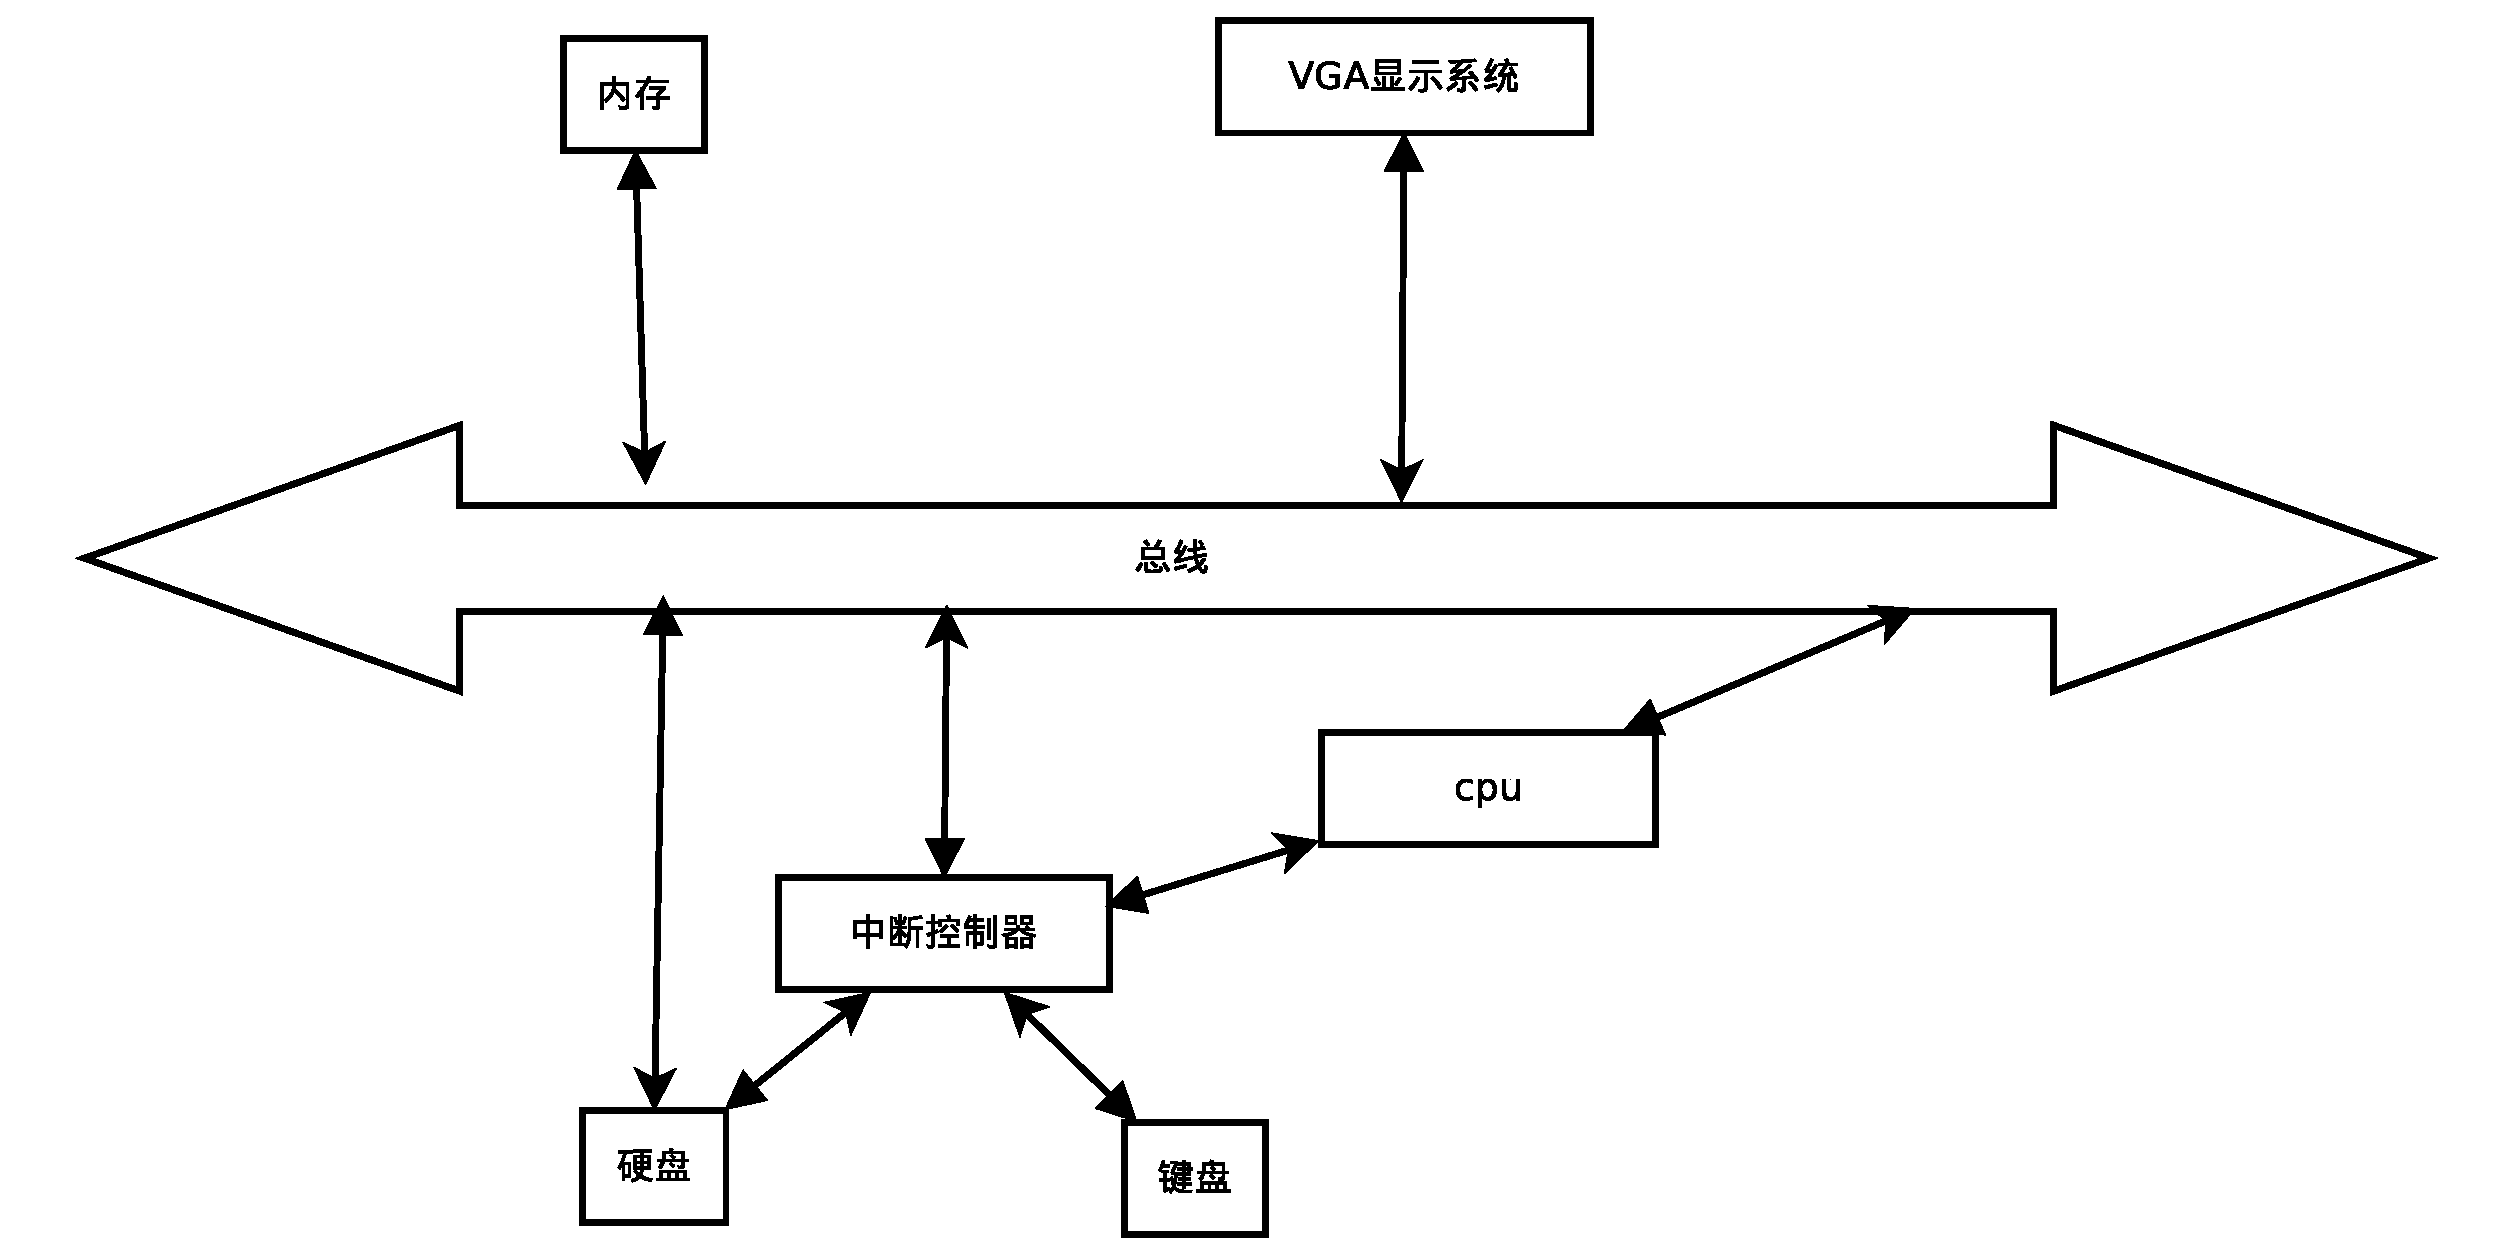
\includegraphics[scale=0.4]{sumti.eps}
\caption{硬件模型}
\end{center}
\paragraph{}
我们所设计的操作系统针对典型的冯诺伊曼计算机。使用总线结构,系统的各部分组件经由总线相互关联在一起。完成交换数据,传递命令等功能。
\subsection{存储系统}
该模型使用三层存储层次。风别为高速缓冲存储器、主存储器、辅助存储器。高速缓冲存储器用来改善主存储器与中央处理器的速度匹配问题。大小和容量对于系统程序员而言是透明的。主存储器是计算机运行时,存储程序和数据的主要场所。在我们的模型中其大小为32MB.而辅助存储器用于扩大存储空间。我们的硬件模型主要有两种类型的辅助存储器。一种是1.44MB大小的软盘。另外一种是ATA硬盘(其大小不固定)。                                                                                     
\subsection{输入输出系统}
像一般的计算机系统一样。该模型使用键盘作为标准输入,也是唯一的输入设备。而将显示器作为输出设备。其中在我们假设显示系统为典型的VGA系统。
\subsection{中央处理器}
这是计算机硬件模型的核心部件。是程序运行的地方。我们的模型使用80386架构的32位CPU。对于设计操作系统而言我们更关心的是他的寄存器环境。

\begin{center}
\label{80386}
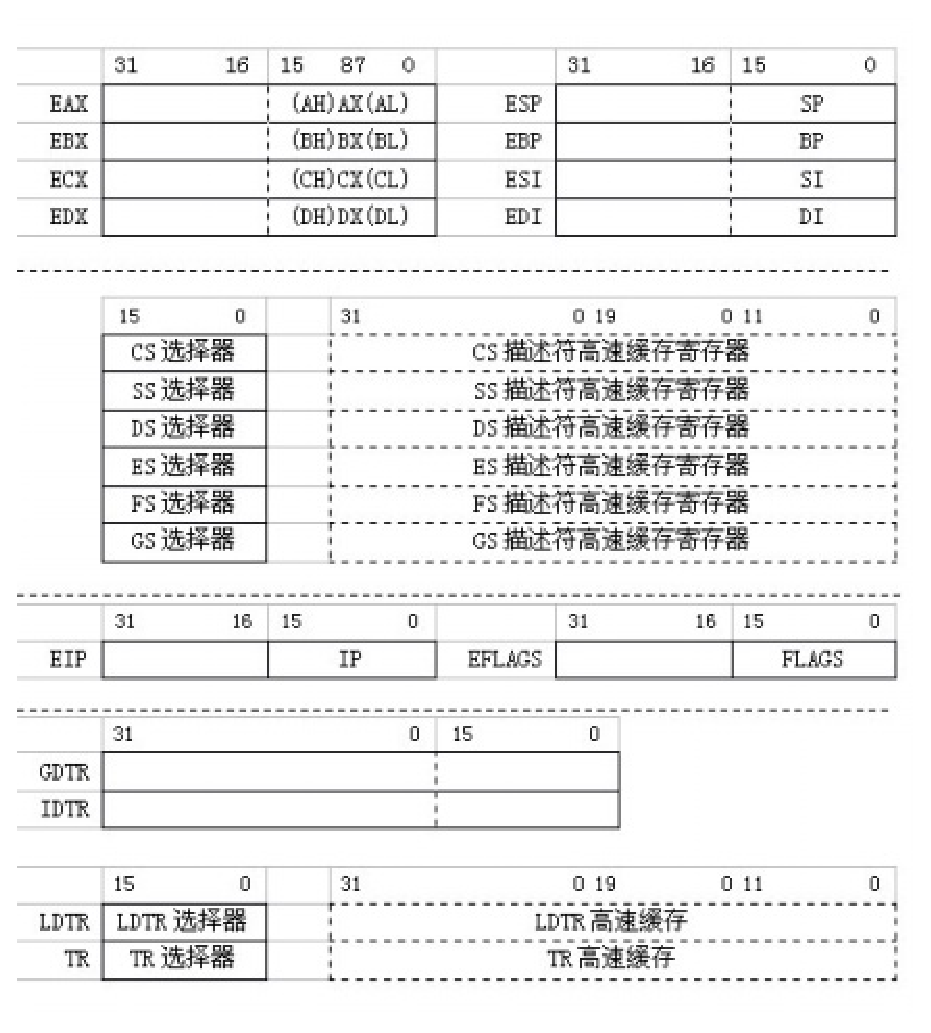
\includegraphics[scale=0.7]{80386.eps}
\end{center}

\subsection{终端控制器}
现在的计算机硬件系统,为了提高信息交换的效率大都采用了中断。采用了中断后,CPU无需空转去等待某个事件的发生。当某个事件发生时向CPU发出一个中断请求信号即可。中断一般用来进行同步操作、实现实时处理、故障处理等功能。而在我们所设计的操作系统中,中断充当了一个浓墨重彩的角色。硬件系统通过两个中断控制器(主8059A、从8259A)来处理来自键盘、硬盘等的各种事件信息。
\begin{center}
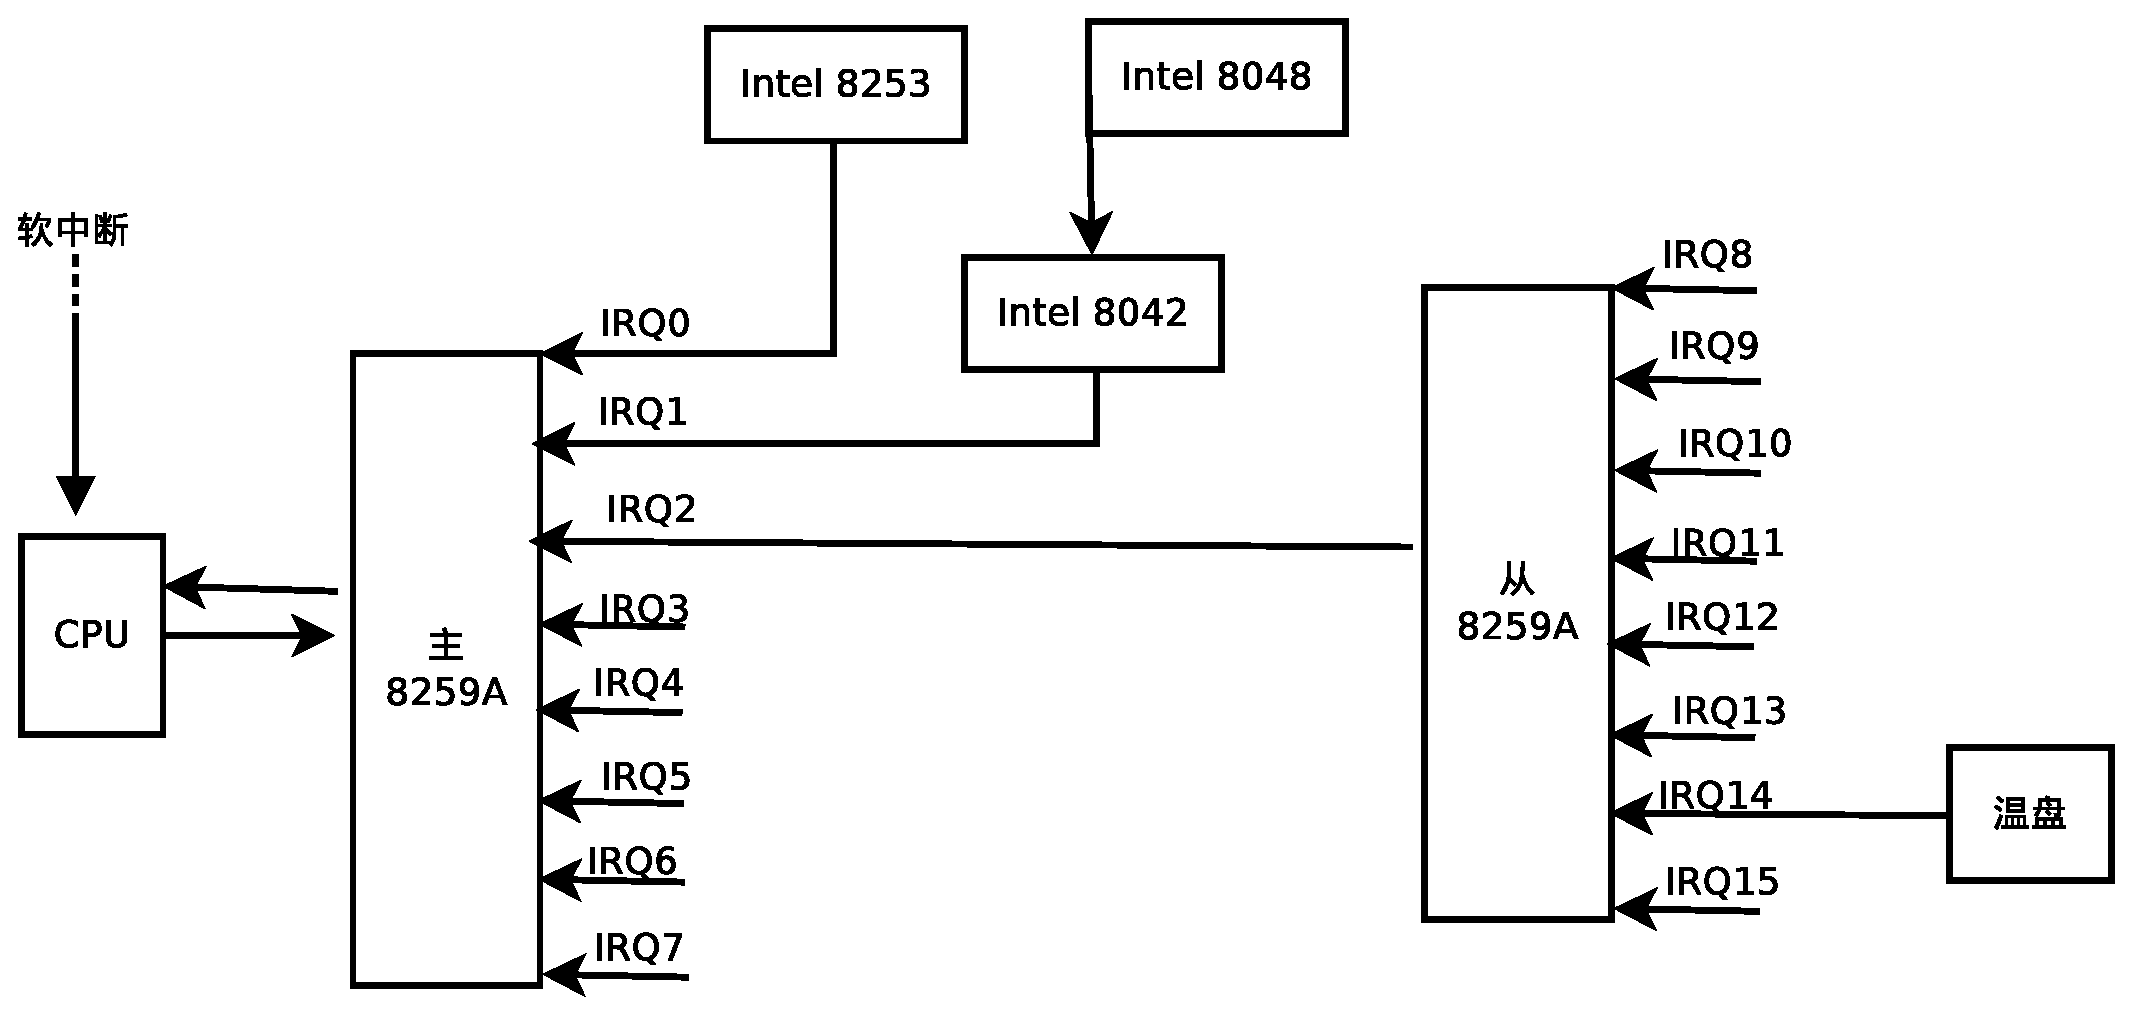
\includegraphics[scale=0.4]{interrupt.eps}
\end{center}
\section{系统启动顺序}
当计算机电源被打开时,他会先进行家电自检(POST),然后寻找启动盘。在我们所设计的系统中,将启动盘设置为软盘。计算机将会检查软盘的0面0磁道1扇区。如果他以0xAA55结束,则BIOS将其识别为一个引导扇区,并将这512B的内容复制到内存地址0000:7c00处,然后跳转到0000:7c00处将控制权彻底交给这段引导代码。到此为止,计算机将不再由BIOS中固有的程序来控制,而变成由我们所设计的错做系统的一部分来控制。
由于存储介质的限制,一般操作系统的引导信息只能存储在前512B之内。因此我们不能将一个完整的操作系统内核安放在这非常小的512B之内。因此我们需要一个专门的程序来引导内核,我们称这个程序为loader。而且在加载内核之前,我们还需要设置好内核的运行环境(内存环境和相应寄存器环境),以及为内核准备一些数据。这些工作也又loader来完成。这样下来,一个完成后的loader所占用的存储空间将超过512B,因此也不能安放在那512B的引导扇区之上。于是我们又需要编写一个程序来引导loader,我们称这个程序为boot。而在加载完成内核之后,才能够运行各种用户程序。于是我们所设计的操作系统的引导顺序如下图所示:

\begin{center}
\label{80386}
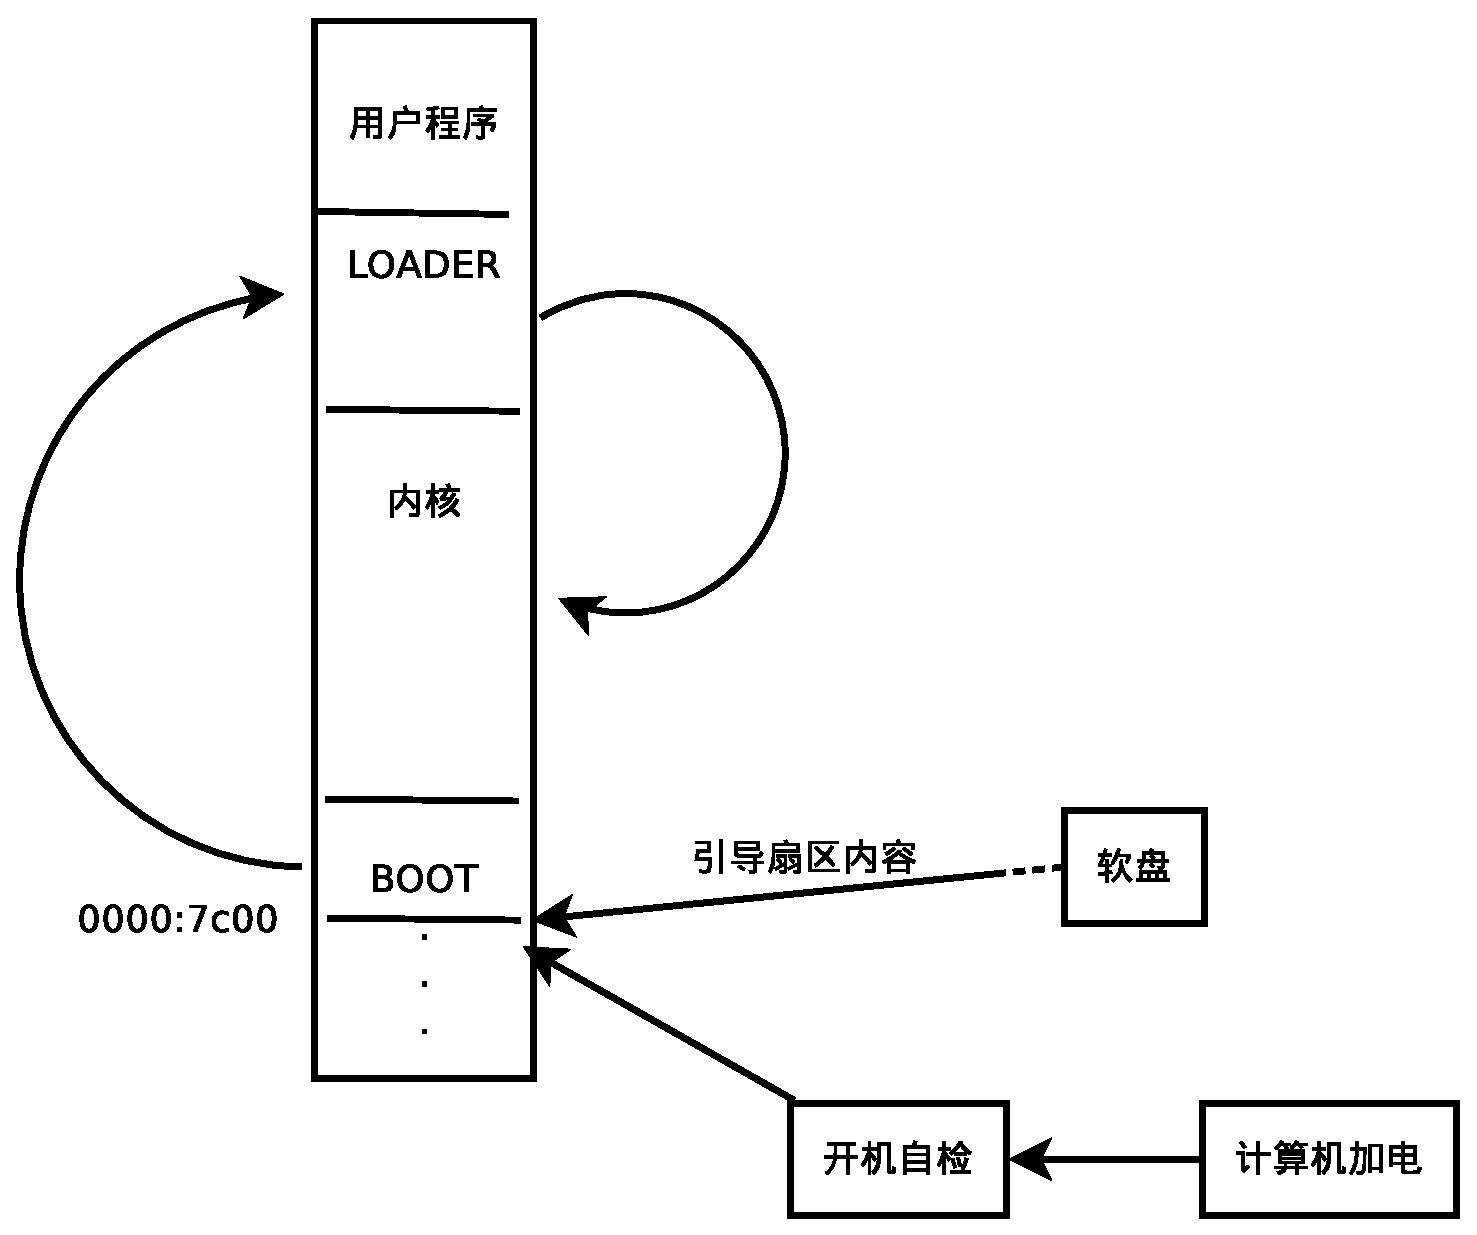
\includegraphics[scale=0.4]{start.eps}
\end{center}

\section{内核结构}
该系统使用微内核结构。微内核结构是一种能够提供必要服务的操作系统内核;其中这些必要的服务包括进程管理,交互进程通信(IPC,Inter-Process Communication)等等。所有服务(包括设备驱动)在用户模式下运行,而处理这些服务同处理其他的任何一个程序一样。因为每个服务只是在自己的地址空间运行。所以这些服务之间彼此之间都受到了保护。微内核是内核的一种精简形式。将通常与内核集成在一起的系统服务层被分离出来,变成可以根据需求加入的选件,这样就可提供更好的可扩展性和更加有效的应用环境。使用微内核设计,对系统进行升级,只要用新模块替换旧模块,不需要改变整个操作系统。而我们所涉及的操作系统整个框架看起来像下图所示:
\begin{center}
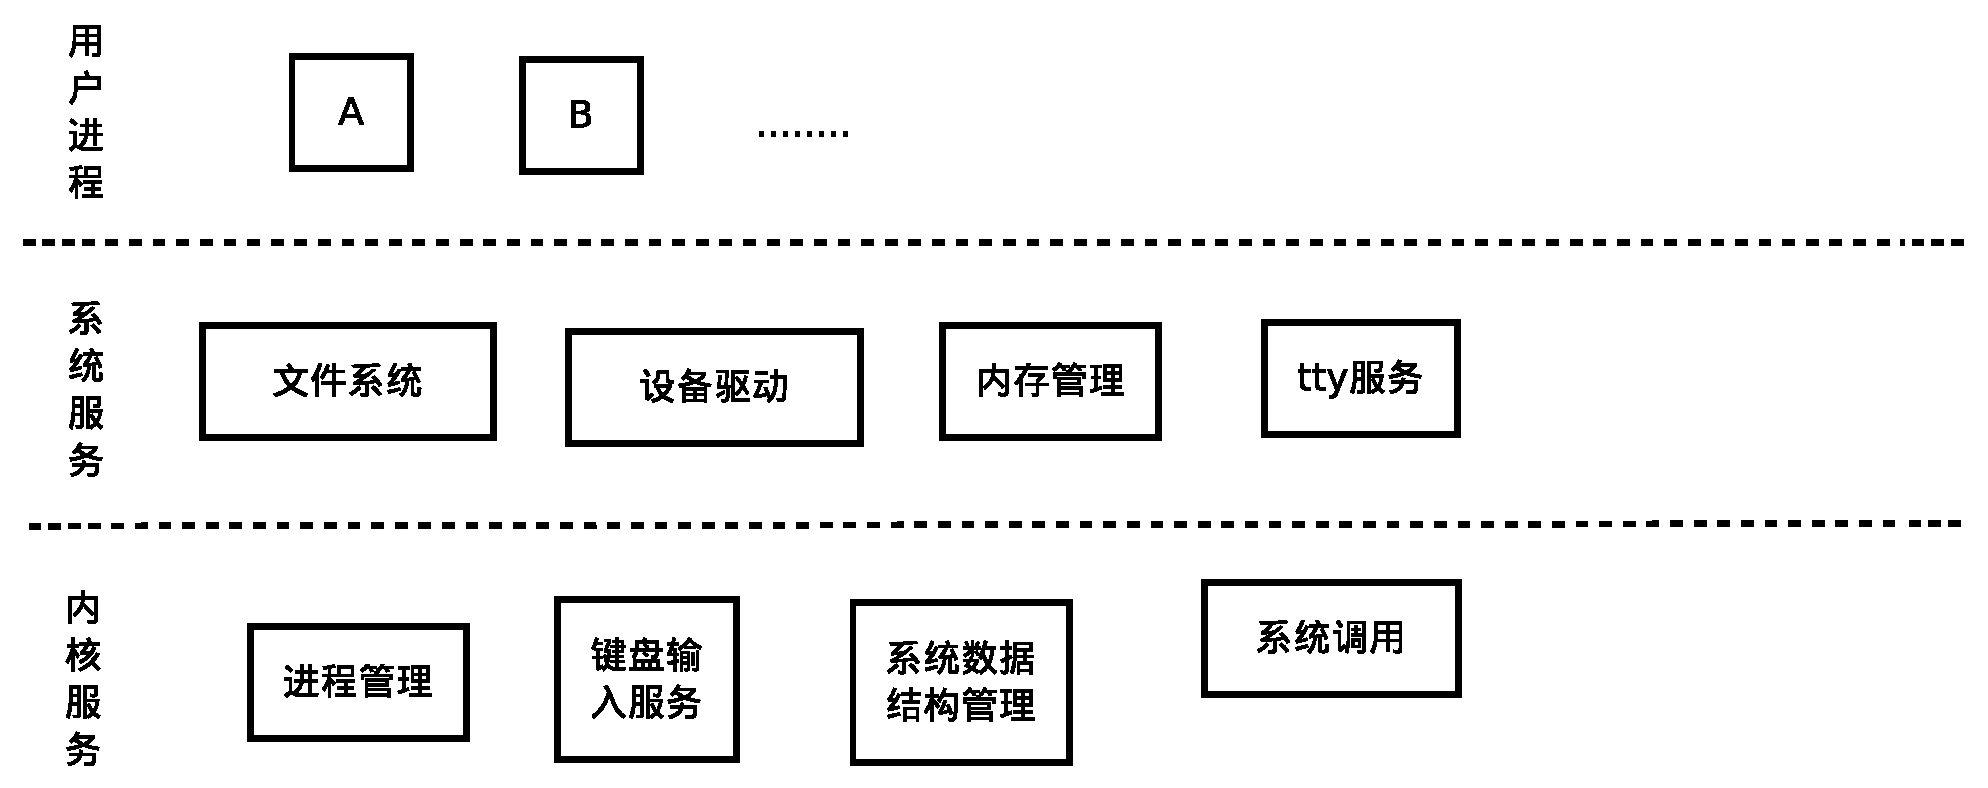
\includegraphics[scale=0.4]{osstruct.eps}
\end{center}

\chapter{具体服务设计}
\section{Boot}
\section{Loader}
\section{中断服务系统}
\subsection{硬件环境}

\subsection{终端服务程序}
\subsection{系统调用}
\section{进程管理}
\section{进程间通信同步IPC}
\section{内存管理}
\section{文件系统}
\section{输入输出系统}
\chapter{进程管理详细设计和实现}

\end{document}
